\chapter{Konzept}
Im Folgenden werden die verschiedenen Funktionsmerkmal des Funktionsgenerators erläutert.
Anschließend wird sein Konzept anhand des grundlegenden Aufbaus des Funktionsgenerators erklärt.
 
\section{Funktionsmerkmale} \label{Concept:Feature}
In diesem Abschnitt wird geschildert, was der Generator leisten kann und wie er sich konfigurieren lässt. 

\subsection{Funktionen} \label{Concept:Feature:Func}
Der Generator kann auf vier verschiedene Funktionsbausteine zurückgreifen, die jeweils einen anderen Spannungsverlauf ausgeben:

\begin{enumerate}
   \item \textbf{Konstante Funktion} \\ 
    Die konstante analoge Spannung \analog{high} liegt am Ausgang an.
  \item \textbf{Rechteck-Funktion} \\
    Der Wert wechselt zwischen \analog{high} und \analog{low} in der Frequenz $f$.
    Der Anteil der Zykluszeit $T$, in dem der Ausgang auf \analog{high} ist, wird über den Parameter dutycycle eingestellt.
    Die Dauer des \analog{high}-Pegels bzw. \analog{low}-Pegels, $T_{h}$ und $T_{l}$ berechnen sich folgendermaßen:
    \begin{align}
      T_{l} &= T \cdot \frac{dutycycle}{255}, dutycycle \in \{0, 1, ..., 255\} \label{Concept:Feature:Func:eqdc1} \\
      T_{h} &= T - T_{l} \label{Concept:Feature:Func:eqdc2}
    \end{align}
    Auf diese Art lassen sich Rechteck-Signale mit einstellbarer Pulsweite erzeugen.
    Diese sogenannten PWM-Signale (``\textbf{P}uls \textbf{W}eiten \textbf{M}odulation'') werden in vielen technischen Anwendungen verwendet.
  \item \textbf{Zick-Zack-Funktion} \\
    Der Analogwert steigt von \analog{low} bis \analog{high} linear an, erreicht er \analog{high}, fällt der Analogwert wieder kontinuierlich auf \analog{low} ab. Somit schwankt der Ausgangspegel mit der Frequenz $f$.
  \item \textbf{Rampen-Funktion} \\
    Der Analogwert wächst, wie bei der Zick-Zack-Funktion, linear bis auf \analog{high} an, danach fällt er aber auf \analog{high} zurück.
    Alternativ kann die Rampe auch von \analog{high} her abfallen und bei Erreichen von \analog{low} wieder auf \analog{high} zurück springen.
\end{enumerate}

\begin{figure}[h] \centering
  {
    \pgfplotsset{
    xtick={0, 15, 30, 45, 60, 75, 90},
    ytick={0, 0.55, 1.1, 1.65, 2.2, 2.75, 3.3},
    xmin=0, xmax=90,
    ymin=-0.2, ymax=3.5,
    % xlabel=$t$,
    xticklabels={$0$, , $T$, , $2T$, , $3T$,}, % \pgfmathprintnumber{\tick}},
    yticklabels={},
    grid=major,
    width=0.52\textwidth,
    height=0.4\textwidth}
  % constant
  \subfloat[][konstante Funktion]{ 
    \begin{tikzpicture}
      \begin{axis}[yticklabels={$h$, , , , , ,$l$}, ylabel=$U(t)$]
        \addplot[color=blue] coordinates{(0, 1.75)(90, 1.75)};
      \end{axis}
    \end{tikzpicture}
    \label{Concept:Plot:const}
  } 
  % square
  \subfloat[][Rechteckfunktion]{
    \begin{tikzpicture}
      \begin{axis}
        \addplot[color=blue]  coordinates{(0, 0)(15, 0)(15, 3.3)(30, 3.3)(30, 0)(45, 0)(45, 3.3)(60, 3.3)(60, 0)(75, 0)(75, 3.3)(90, 3.3)};
      \end{axis}
    \end{tikzpicture}
    \label{Concept:Plot:square}
  } 

  % zigzag \foreach \x in {0, 15, ..., 90} {(\x, 3.3)}
  \subfloat[][Zick-Zack-Funktion]{
    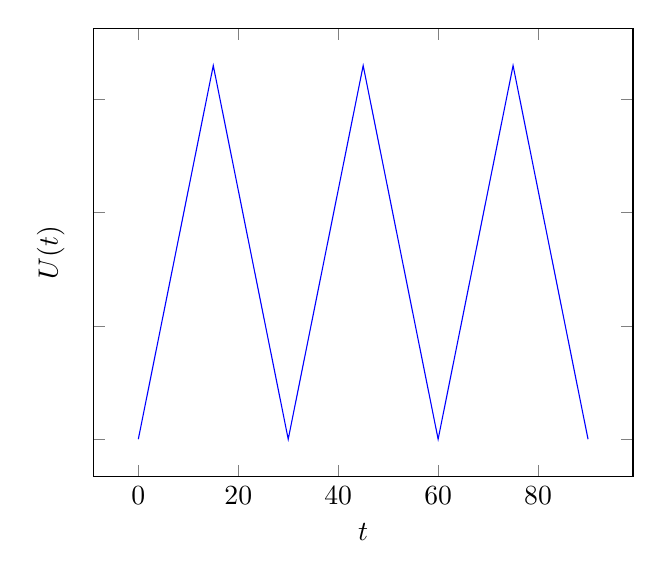
\begin{tikzpicture}
      \begin{axis}[yticklabels={$h$, , , , , ,$l$}, ylabel=$U(t)$, xlabel=$t$]
        \addplot[color=blue] coordinates{(0, 0)(15, 3.3)(30, 0)(45, 3.3)(60, 0)(75, 3.3)(90, 0)};
      \end{axis}
    \end{tikzpicture}
    \label{Concept:Plot:zigzag}
  }
  % ramp
  \subfloat[][Rampenfunktion]{
    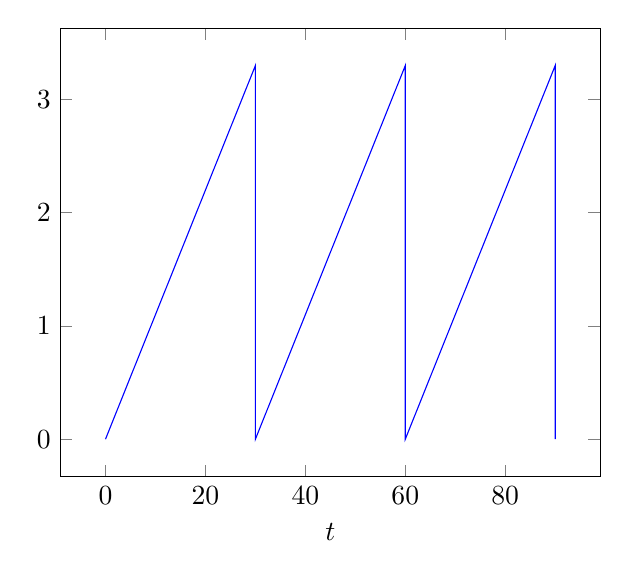
\begin{tikzpicture}
      \begin{axis}[xlabel=$t$]
        \addplot[color=blue, domain=0:90]  coordinates{(0, 0)(30, 3.3)(30, 0)(60, 3.3)(60, 0)(90, 3.3)(90, 0)};
      \end{axis}
    \end{tikzpicture}
    \label{Concept:Plot:ramp}
  }
  \caption{Funktionen, die der Funktionsgenerator ausgeben kann. Ihr Verlauf ist als Spannung $U(t)$ über der Zeit $t$ aufgetragen. Die Zykluszeit und \analog{high} bzw. \analog{low} sind durch  $T$, $h$ und $l$ gekennzeichnet.} \label{Concept:Plot}
\end{figure}

\subsection{Konfiguration}
Der Funktionsgenerator muss, um extern konfiguriert werden zu können, über eine Möglichkeit für Nutzereingaben verfügen.
Zu diesem Zweck wird die UART-Schnittstelle auf dem Basys 3-Board genutzt.
Über diese kann der Nutzer Konfigurationsbefehle per Computer versenden, die dann vom Generator interpretiert werden.
Darüber hinaus nutzerseitig wurde ein Python-Script geschrieben, das die Kommunikation mit dem Generator vereinfacht.

\section{Aufbau}
Der Funktionsgenerator ist aus verschiedenen Einzelkomponenten zusammengesetzt.
Ihre Verschaltung im Generator ist in \cref{Concept:FuncGenDia} zu sehen.
In der Abbildung kann man gut erkennen, dass die verschiedenen Funktionen parallel arbeiten und von der Konfigurationsschnittstelle mit den Signalen \bitvect{cyc\_ticks}, \bitvect{high}, \bitvect{low}, \bitvect{thresh} und \bitvect{direction} gesteuert werden.
Das Signal \bitvect{waveform} steuert den Multiplexer, der das Ausgabesignal \bitvect{y\_out} an die interne Schnittstelle des DAC-Wandlers weitergibt.
Diese Schnittstelle generiert daraus die Signale \lowactive{SYNC}, \bit{DINA}, \bit{DINB} und \bit{CLK} und transferiert sie dann an den DAC-Wandler.
Dieser wandelt sie anschließend in ein analoges Signal um.

\begin{figure}[h] \centering
  \includegraphics[width=1.0\textwidth, angle=-90, origin=c]{function_generator}
  \caption{Diagramm des Funktionsgenerators. Aus Gründen der Übersichtlichkeit sind die \bit{CLK} Signale und \lowactive{CE} Signale nicht angeschlossen dargestellt. Alle \bit{CLK} Signale sind an den Systemtakt angeschlossen und alle \lowactive{CE} Signale liegen auf Masse.}  \label{Concept:FuncGenDia}
\end{figure}

